\documentclass[12pt, a4paper, twoside]{article}
\usepackage[margin=1in, headheight=0.3in, headsep=0.2in]{geometry}
\textwidth 16.5 cm \textheight 24cm
\oddsidemargin -2mm

% Packages
\usepackage{amsmath, listings, xcolor, tcolorbox, microtype, fancyhdr, hyperref, tikz, float}
\usetikzlibrary{decorations.pathreplacing}

% Configure text justification
\raggedbottom
\renewcommand{\textfraction}{0.05}
\renewcommand{\floatpagefraction}{0.85}
\renewcommand{\topfraction}{0.9}

% Configure the header
\setlength{\headheight}{14.49998pt}
\pagestyle{fancy}
\fancyhf{} 
\fancyhead[L]{\leftmark}
\fancyhead[R]{\thepage}
\renewcommand{\footrulewidth}{0pt}
\renewcommand{\sectionmark}[1]{\markboth{\thesection.~#1}{}}
\renewcommand{\subsectionmark}[1]{}

% Configure the links to look professional
\hypersetup{
    colorlinks=true,      % false: boxed links; true: colored links
    linkcolor=navyblue,   % Color of internal links (TOC, sections)
    citecolor=navyblue,   % Color of citations
    urlcolor=navyblue,    % Color of external URLs
    pdftitle={Numerical Solutions using RK5},  % Metadata for the PDF
    pdfauthor={Mohak Das}                      % Metadata for the PDF
}

% Define custom colors for code
\definecolor{codegreen}{rgb}{0,0.6,0}
\definecolor{codegray}{rgb}{0.2,0.2,0.2}
\definecolor{codepurple}{rgb}{0.58,0,0.82}
\definecolor{backcolour}{rgb}{0.95,0.95,0.92}
\definecolor{navyblue}{RGB}{0, 51, 102} % A professional deep blue

% Configure the Fortran style
\lstdefinestyle{codestyle}{
    backgroundcolor=\color{backcolour},   
    commentstyle=\color{codegreen},
    keywordstyle=\color{magenta},
    numberstyle=\tiny\color{codegray},
    stringstyle=\color{codepurple},
    basicstyle=\ttfamily\footnotesize, % Typewriter font, small size
    breakatwhitespace=false,         
    breaklines=true,                 % Break long lines automatically
    captionpos=b,                    % Caption at bottom
    keepspaces=true,                 
    numbers=left,                    % Line numbers on the left
    numbersep=5pt,                  
    showspaces=false,                
    showstringspaces=false,
    showtabs=false,                  
    tabsize=4,
    language=Fortran                 % Set language to Fortran
}

\begin{document}

    \begin{titlepage}
        \centering

        \vspace*{\fill}
        \Huge \textsc{\textcolor{navyblue}{Jadavpur University}}\\
        \LARGE \textsc{Department of Physics}\\[1cm]

        \textcolor{navyblue}{\rule{\linewidth}{0.8mm}} \\[0.4cm] 
        \Huge \textbf{\textcolor{navyblue}{Numerical Solutions of System \\ of Non-linear ODE using the \\ Runge-Kutta Method}} \\[0.2cm]
        \textcolor{navyblue}{\rule{\linewidth}{0.8mm}} \\[1.5cm] 

        \large \textit{The Lorenz System}\\[0.5cm]

        \begin{tcolorbox}[colback=navyblue!5!white, colframe=navyblue, width=0.8\textwidth, boxrule=0.5mm, arc=2mm, auto outer arc]
            \Large
            $$
            \begin{aligned}
            \dot{x} &= \sigma(y-x) \\
            \dot{y} &= x(\rho-z)-y \\
            \dot{z} &= xy-\beta z
            \end{aligned}
            $$
        \end{tcolorbox}

        \vspace{1.5cm}

        \noindent
        \begin{minipage}{0.4\textwidth}
            \begin{flushleft} \Large
                \textbf{Submitted by:}\\
                \textcolor{navyblue}{Mohak Das}\\
            \end{flushleft}
        \end{minipage}
        \begin{minipage}{0.4\textwidth}
            \begin{flushright} \Large
                \textbf{Supervisor:} \\
                Dr. Suvankar Ray\\
                \vspace{0.6cm}
            \end{flushright}
        \end{minipage}
        \vspace{1cm}

        \textbf{Class:} PG-I\\
        \textbf{Class Roll No:} 002520702028\\
        \textbf{Exam Roll No:} PPHD0261034
        \vspace{1.5cm}

        \textsc{Computational Physics Lab}

        \vspace*{\fill}


    \end{titlepage}
    \thispagestyle{empty}

    \begin{abstract}
        This report computationally investigates the phase space dynamics of six distinct non-linear systems to explore phenomena ranging from competitive exclusion to deterministic chaos. A custom 5th-order Runge-Kutta (RK5) numerical solver was implemented in Fortran 90 to integrate the governing coupled differential equations, with Gnuplot utilized for high-fidelity phase portrait and vector field visualizations. The analyzed models span a wide topological spectrum, including the simple pendulum, asymmetric and symmetric Lotka-Volterra competition models (Rabbit-Sheep and Bacterial Colony), a pure quartic oscillator, a mixed saddle-centre topology, and the chaotic Lorenz system. The study highlights the profound influence of phase space geometry on system evolution, visualizing how separatrices govern survival in symmetric competition, how periods become heavily amplitude-dependent in purely non-linear potentials, and how strange attractors emerge from deterministic equations. Furthermore, the application of a uniform RK5 solver exposes critical computational nuances, underscoring the necessity of boundary conditions for unbounded, escaping trajectories and demonstrating the inherent limitations of non-symplectic integrators when modeling strictly conservative systems.
    \end{abstract}
    
    \thispagestyle{empty}
    \newpage

  	\tableofcontents
	\thispagestyle{empty}
	
	\clearpage
	\pagenumbering{arabic}
    \section{Introduction}
        Non-linear dynamics provides the mathematical framework for understanding complex systems whose evolution over time is not strictly proportional to their current state. While linear systems yield predictable, easily solvable harmonic behaviors, non-linear systems exhibit a rich tapestry of phenomena ranging from multiple equilibrium states and competitive exclusion to purely non-linear oscillations and deterministic chaos.

        The primary objective of this assignment is to computationally investigate and visualize the phase space trajectories of various coupled differential equations. To achieve this, a custom 5th-order Runge-Kutta (RK5) numerical solver was implemented in Fortran 90. Although the choice of integration scheme was left open for this assignment, RK5 was specifically selected to be used across all problems due to its high degree of accuracy and robust local error control. This solver was utilized to integrate the equations of motion over time, while Gnuplot was employed to render the resulting phase portraits and vector flow fields.

        This report systematically analyzes six distinct dynamical regimes:
        \begin{enumerate}
            \item {\bf The Simple Pendulum:} Illustrating the fundamental transition from linear harmonic approximation at small angles to non-linear anharmonic motion at larger amplitudes.
            \item {\bf Asymmetric Population Dynamics (Rabbit-Sheep Model):} Demonstrating the standard Lotka-Volterra competition model with uneven resource competition and intrinsic growth rates.
            \item {\bf Symmetric Population Dynamics (Bacterial Colony):} Highlighting a perfectly balanced competitive model where survival is dictated entirely by initial conditions, leading to competitive exclusion governed by a distinct separatrix.
            \item {\bf Purely Non-Linear Systems (Quartic Oscillator):} Revealing bounded orbits in a potential ($V \propto x^4$) where periods are heavily amplitude-dependent and standard linear stability analysis fails.
            \item {\bf Mixed Topology Systems (Saddle-Centre):} Showcasing a hybrid system containing both linear and non-linear terms, yielding the simultaneous coexistence of a stable topological centre, an unstable saddle point, and trajectories that escape to infinity.
            \item {\bf The Lorenz System:} Providing a classic, three-dimensional demonstration of deterministic chaos, strange attractors, and extreme sensitivity to initial conditions (the butterfly effect).
        \end{enumerate}

    \section{Numerical Implementation}
        \subsection{Global Constants and Precision}
        To ensure numerical stability and physical consistency across all problems, a shared module \texttt{constants\_mod} is used. This module defines the double-precision floating-point kind (\texttt{real64}) and defines the value of $\pi$ and gravitational acceleration $g$.
        \lstinputlisting[style= codestyle]{src/shared/constants_mod.f90}

        \subsection{The General RK5 Solver}
        The numerical integration of the governing differential equations was performed using Butcher's fifth-order Runge-Kutta (RK5) method. Unlike the standard fourth-order method, this RK5 scheme evaluates the derivative at six intermediate stages ($k_1$ through $k_6$) within a single time step $h$. The system's state is then advanced using a precisely weighted linear combination of these six slopes. This higher-order approach yields a global truncation error of $\mathcal{O}(h^5)$, providing the strict numerical precision required to accurately resolve the trajectories of non-linear and chaotic dynamic systems without requiring prohibitively small step sizes.
        \lstinputlisting[style= codestyle]{src/shared/RK5_solver.f90} \vspace{0.5cm}
        We have chosen RK5 method over RK4 method due to the following reasons:
        \begin{itemize}
            \item {\bf Slower Error Accumulation in Chaos:} Non-linear systems especially chaotic ones like the Lorenz attractor, exhibit exponential sensitivity to initial conditions. Any tiny numerical truncation error made at step $t$ is amplified exponentially by step $t+1$. RK5's global error scales at $\mathcal{O}(h^5)$ compared to RK4's $\mathcal{O}(h^4)$. By generating a drastically smaller error per step, RK5 significantly delays the inevitable numerical divergence of chaotic trajectories
            \item {\bf Phase Space Fidelity:} In systems like the Simple Pendulum, we are looking at closed loops in phase space (libration). Lower-order methods like RK4 (and especially Euler) suffer from artificial "numerical damping" or energy drift, causing those closed loops to spiral slowly inward or outward over long integration times. RK5 preserves the geometric invariants and total energy of the phase space much more strictly.
            \item {\bf Computational Efficiency:} While RK5 requires six function evaluations per step compared to RK4's four, the massive increase in accuracy allows us to use a noticeably larger step size $h$ while maintaining the same error tolerance. Taking fewer, slightly heavier steps is almost always faster than taking millions of tiny steps.
        \end{itemize}

    \section{Solution to the Assignment Problems}
        \subsection{Problem 1: Simple Pendulum}
        \begin{itemize}
            \item {\bf Description: }The simple pendulum is a fundamental model in classical mechanics consisting of a mass suspended from a pivot. While small oscillations can be approximated linearly, the true equation of motion is non-linear due to the sine term, leading to complex phase space trajectories like the "eye" shapes (libration) and wavy lines (rotation).
            \item {\bf The Equation of Motion: }The equation of motion for simple pendulum is given by a non-liner 2nd order differential equation, $$\boxed{\ddot{\theta} + \frac{g}{L} \sin{\theta} = 0}$$
            This can be decomposed in two first order ODE as, \begin{eqnarray*}
            \dot{\theta} & = & \omega \\
            \dot{\omega} & = & -\frac{g}{L} \sin{\theta}
            \end{eqnarray*} where $\theta$ is position and $\omega$ is velocity.
            \item {\bf Code: } \lstinputlisting[style= codestyle]{src/problems/prob01_simple_pendulum.f90}
            \item {\bf GNUplot Command:} \lstinputlisting[style= codestyle]{gnuplot/plot_prob01_simple_pendulum.plt}
            \item {\bf Plot: }\begin{figure}[H]
                \centering
                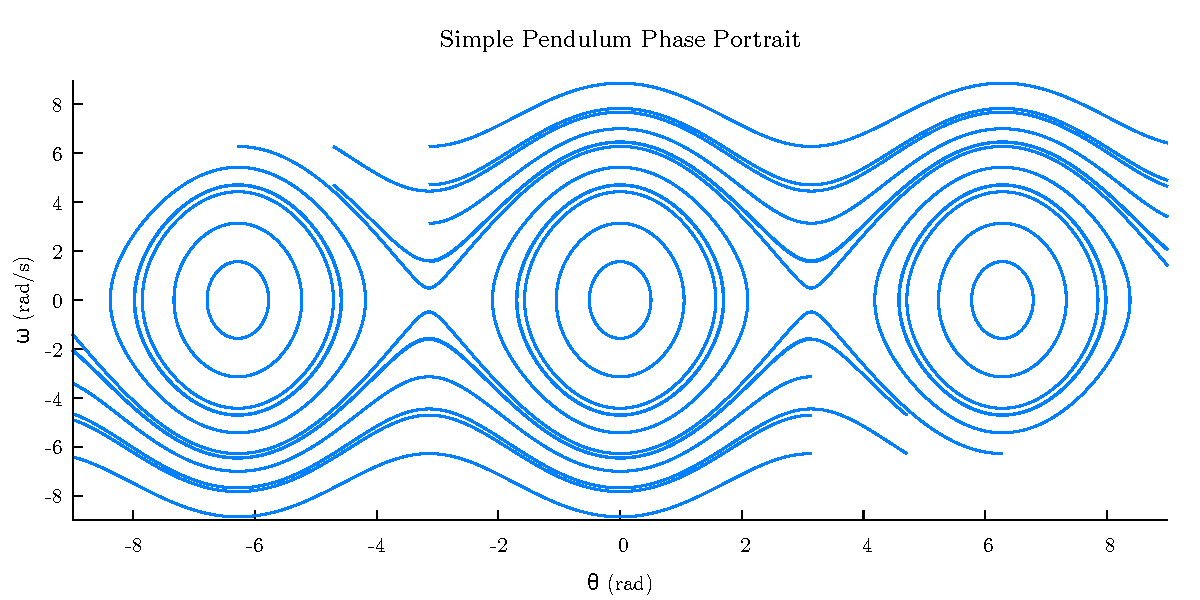
\includegraphics[width=0.8\textwidth]{plots/prob01_simple_pendulum_gnuplot.pdf}
                \label{fig:prob01_simple_pendulum}
            \end{figure}
        \end{itemize}    
        
        \subsection{Problem 2: Lotka-Volterra Competition Model}
        \begin{itemize}
            \item {\bf Description: }Lotka-Volterra Competition Model is a classic population dynamics model describing two species competing for the exact same limited resources (in this case, grass). Unlike the predator-prey version, both species negatively impact each other's growth rates. Depending on the initial population sizes, the phase portrait shows the trajectories flowing toward different stable equilibria where one species ultimately outcompetes the other.
            \item {\bf The Equations: }This model is defined as a coupled system of two 1st-order equations, \begin{eqnarray*}
                \dot{x} & = & x (3 - x - 2y) \\
                \dot{y} & = & y (2 - x - y)
            \end{eqnarray*} where $x$ = rabbit and $y$ = sheep.
            \item {\bf Code: } \lstinputlisting[style= codestyle]{src/problems/prob02_rabbit_sheep_model.f90}
            \item {\bf GNUplot Command:} \lstinputlisting[style= codestyle]{gnuplot/plot_prob02_rabbit_sheep_model.plt}
            \item {\bf Plot: }\begin{figure}[H]
                \centering
                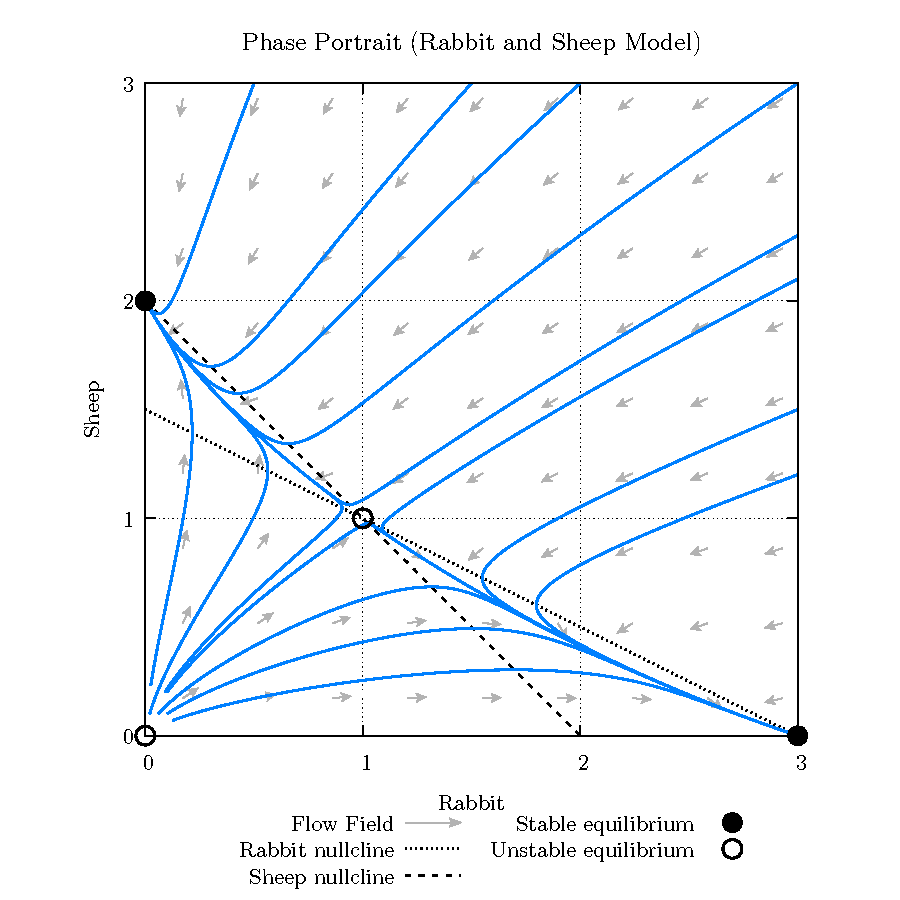
\includegraphics[width=0.8\textwidth]{plots/prob02_rabbit_sheep_model.pdf}
                \label{fig:prob02_rabbit_sheep}
            \end{figure}
        \end{itemize}
        
        \subsection{Problem 3: Lorenz Butterfly}
        \begin{itemize}
            \item {\bf Description: }Originally developed as a highly simplified mathematical model for atmospheric convection, the Lorenz system is one of the most famous examples of deterministic chaos. It demonstrates extreme sensitive dependence on initial conditions (the "butterfly effect").
            \item {\bf The Equations: }This model is defined natively as a system of three coupled 1st-order equations governed by parameters $\sigma$ (Prandtl number), $\rho$ (Rayleigh number), and $\beta$. \begin{eqnarray*}
                \dot{x} & = & \sigma (y - x) \\
                \dot{y} & = & x (\rho - z) - y \\
                \dot{z} & = & x y - \beta z
            \end{eqnarray*} The Lorenz system behaves as a strange attractor primarily when the Rayleigh number ($\rho$) is high, specifically around the classic parameters  $\sigma = 10$, $\rho = 28$, and $\beta=\frac{8}{3}$. In this regime, trajectories are drawn to a fractal, butterfly-shaped structure, never settling into equilibrium or repeating, exhibiting high sensitivity to initial conditions (the butterfly effect)
            \item {\bf Code: } \lstinputlisting[style= codestyle]{src/problems/prob03_lorenz_butterfly.f90}
            \item {\bf GNUplot Command:} \lstinputlisting[style= codestyle]{gnuplot/plot_prob03_lorenz_butterfly.plt}
            \item {\bf Plot: }
            \begin{enumerate}
                \item {Lorenz Attractor: } \begin{figure}[H]
                    \centering
                    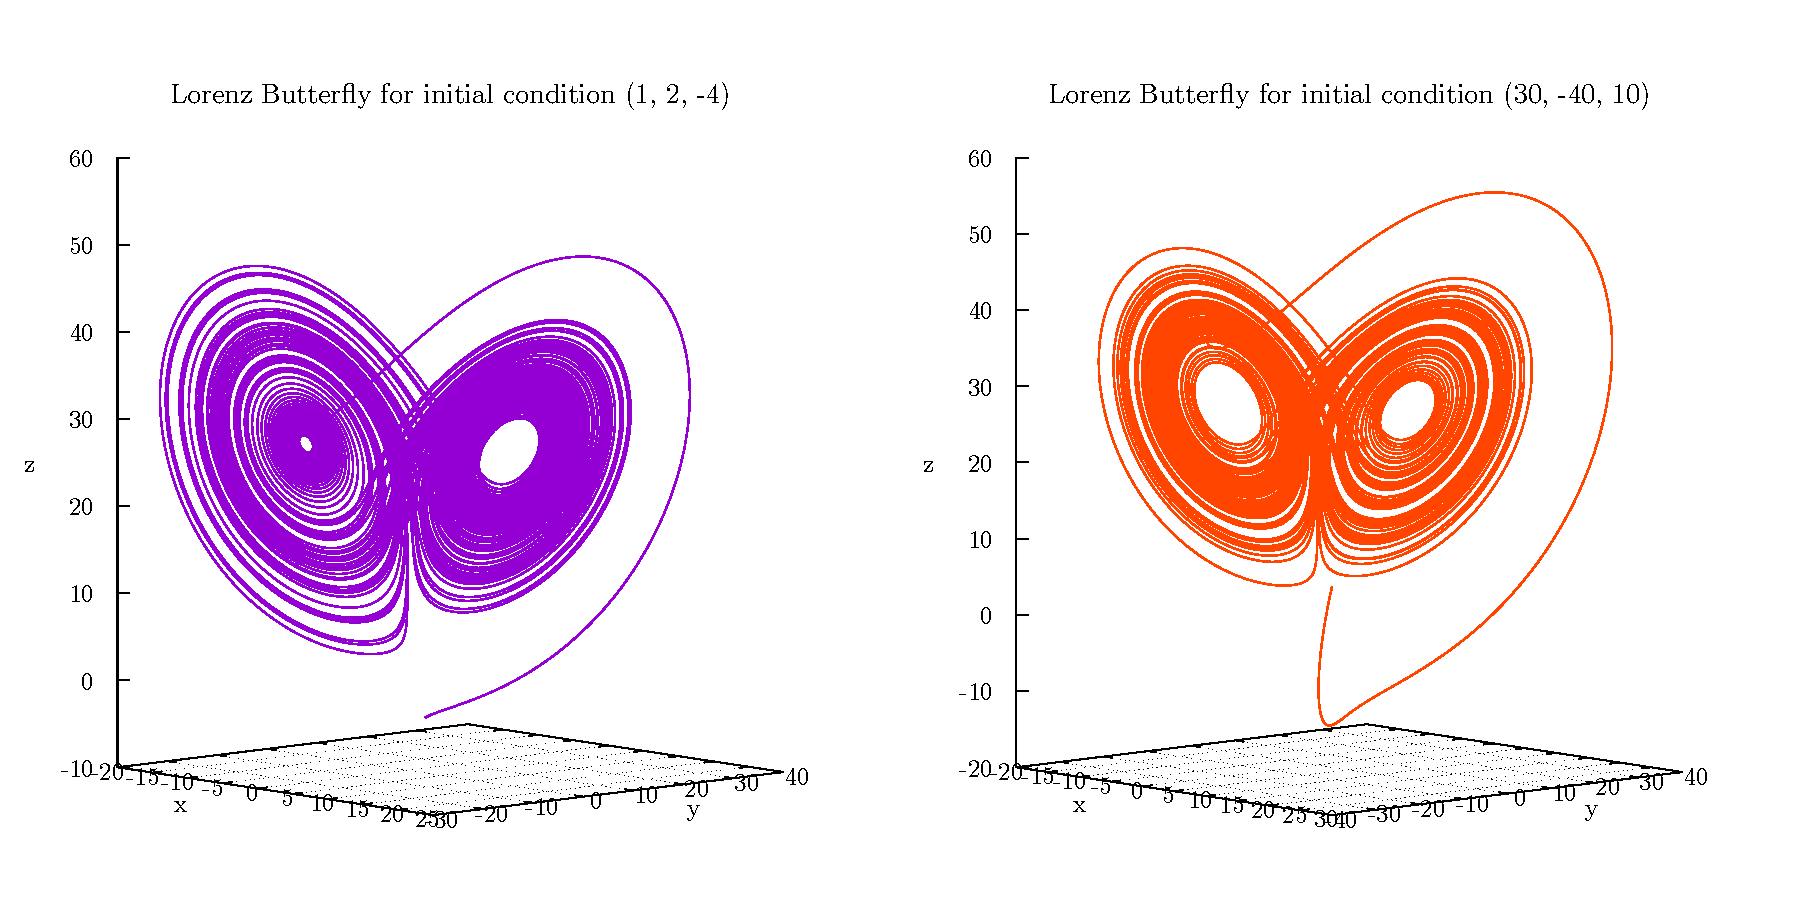
\includegraphics[width=0.8\textwidth]{plots/prob03_1_lorenz_attractor.pdf}
                    \label{fig:prob03_1_lorenz_attractor}
                \end{figure} \vspace{1cm}
                
                \item {Lorenz Attractor (2D Projection, $z$ vs $x$): }
                \begin{figure}[H]
                    \centering
                    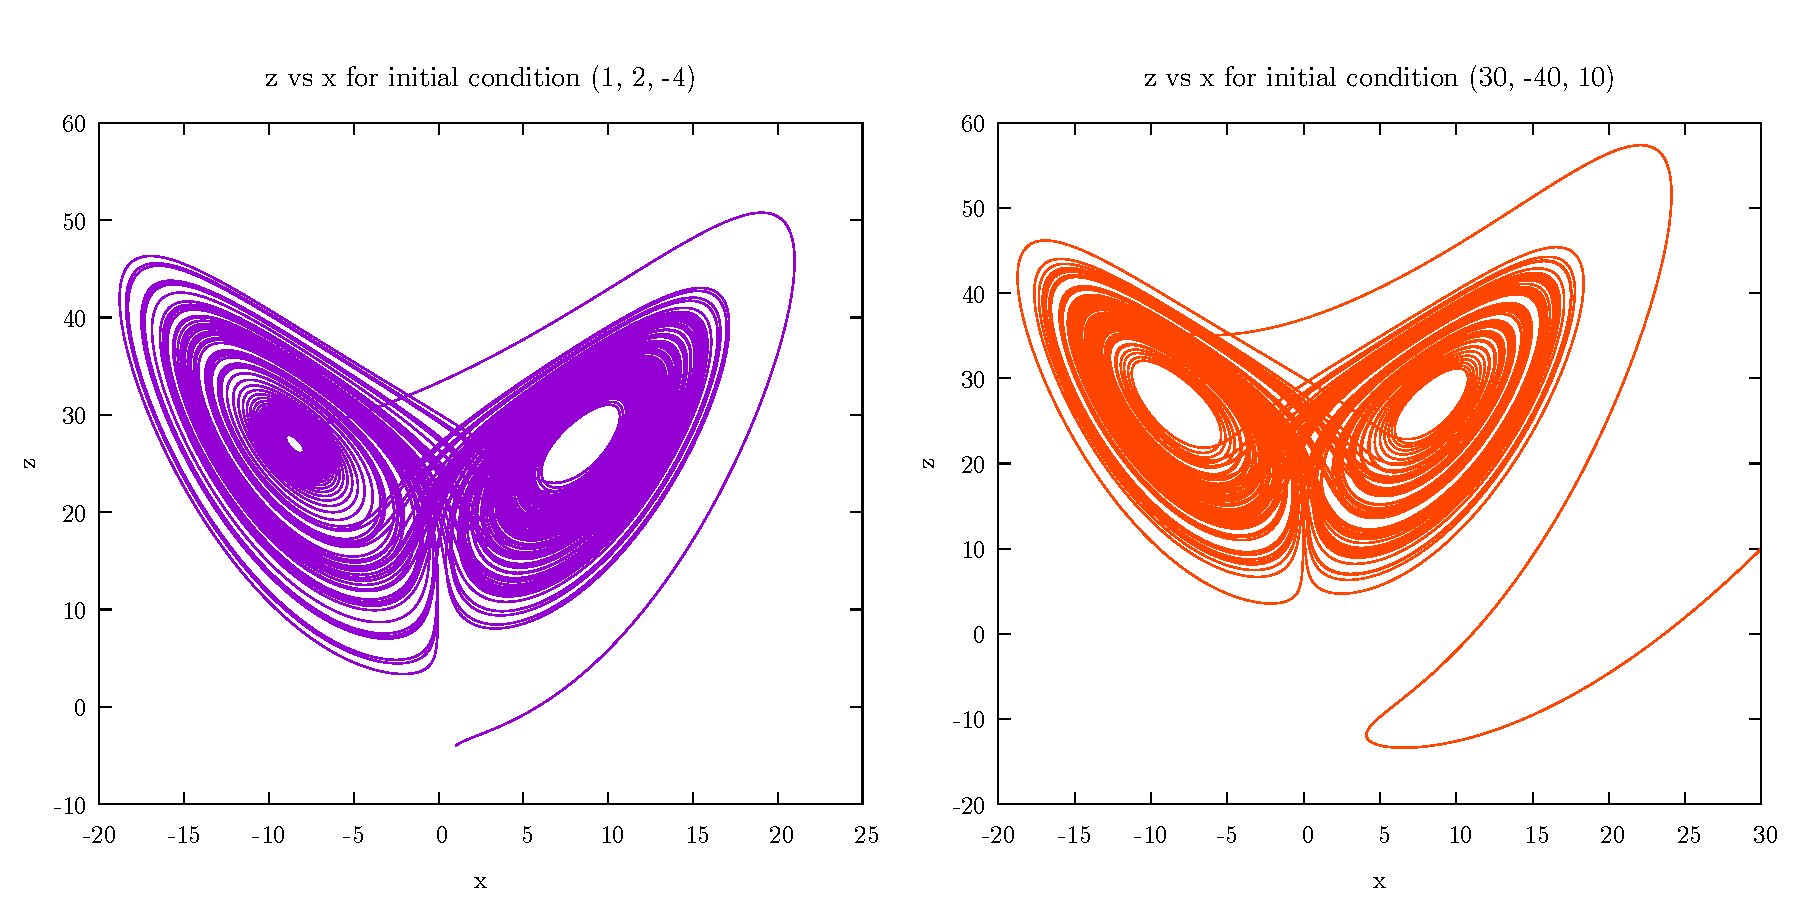
\includegraphics[width=0.8\textwidth]{plots/prob03_2_lorenz_attractor_x_z.pdf}
                    \label{fig:prob03_2_lorenz_attractor_x_z}
                \end{figure} \newpage
                
                \item {Lorenz Attractor (Time Series): } \begin{figure}[H]
                    \centering
                    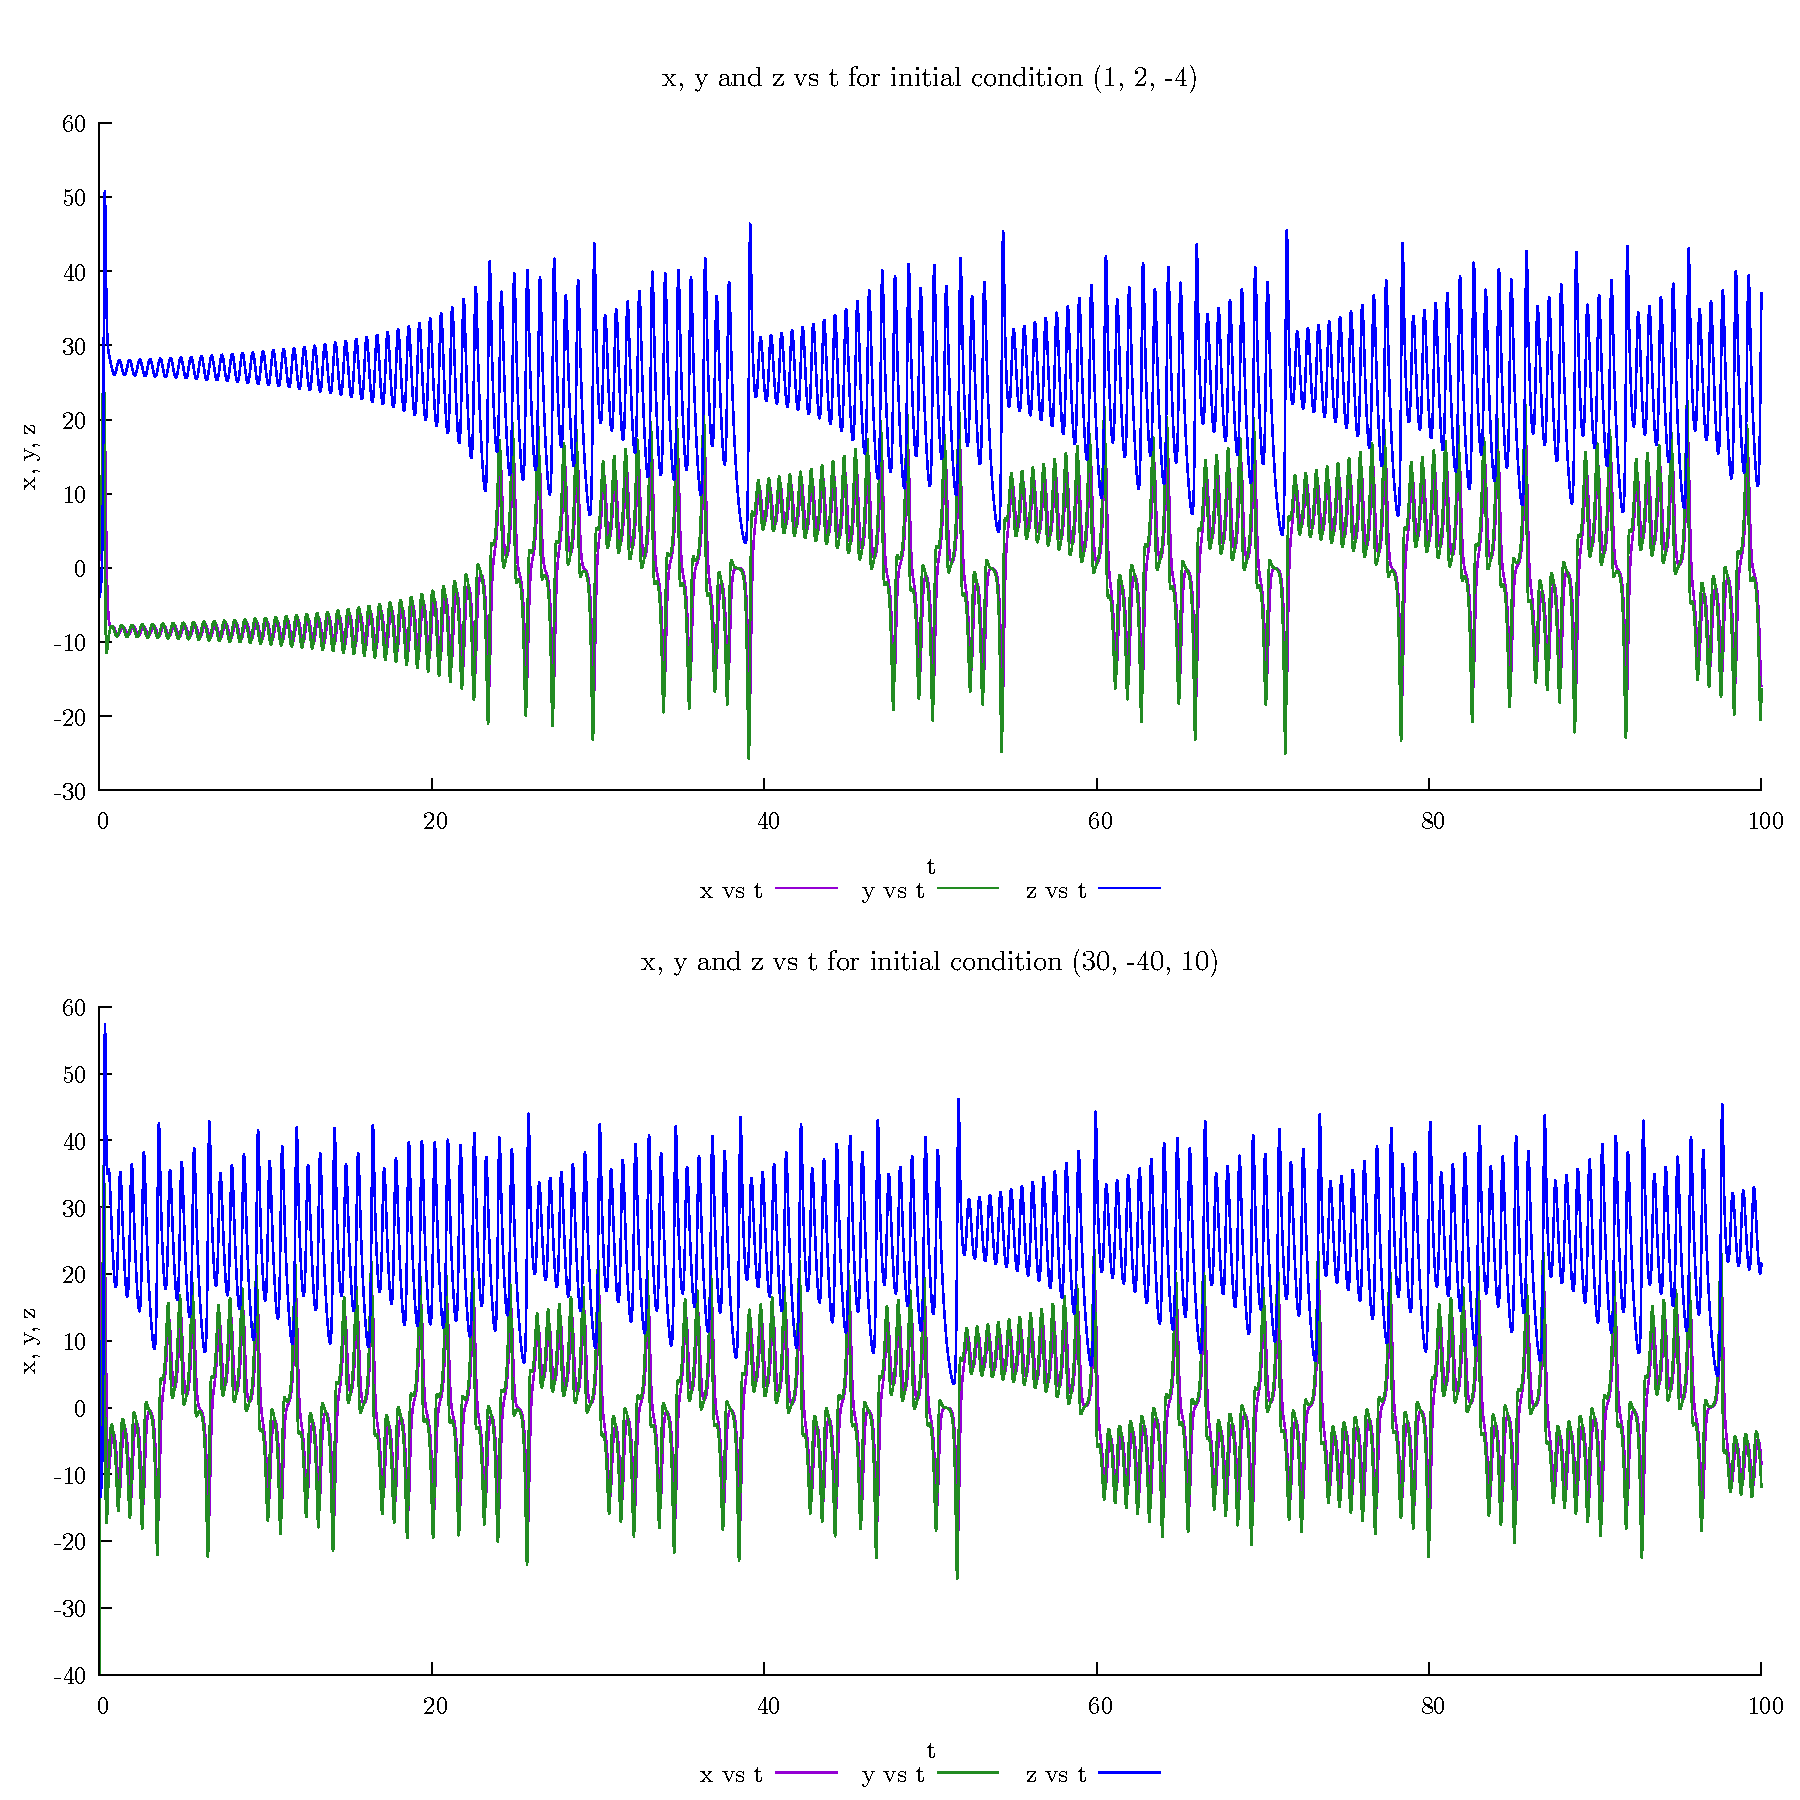
\includegraphics[width=0.9\textwidth]{plots/prob03_3_lorenz_attractor_x_y_z_t.pdf}
                    \label{fig:prob03_3_x_y_z_t}
                \end{figure}
            \end{enumerate}
        \end{itemize}
        
        \subsection{Problem 4: The Symmetric Bacterial Colony}
        \begin{itemize}
            \item {\bf Description: }This system models the population dynamics of two competing bacterial colonies. Unlike the classic asymmetric Rabbit-Sheep model, this system places both species on equal footing. Both colonies share identical intrinsic growth rates and experience the same magnitude of intra-species and inter-species competition. Because the parameters are perfectly symmetric, survival is determined entirely by initial conditions, leading to competitive exclusion governed by a separatrix along the diagonal $y = x$.
            \item {\bf The Equations: }The time evolution of the populations $x$ and $y$ is given by the coupled non-linear differential equations: 
            \begin{eqnarray*}
                \dot{x} & = & = x(3 - x - 2y) \\
                \dot{y} & = & = y(3 - 2x - y)
            \end{eqnarray*}
            \item {\bf Code: } \lstinputlisting[style= codestyle]{src/problems/prob04_bacteria_colony.f90}
            \item {\bf GNUplot Command:} \lstinputlisting[style= codestyle]{gnuplot/plot_prob04_bacteria_colony.plt}
            \item {\bf Plot: } 
            \begin{figure}[H]
                \centering
                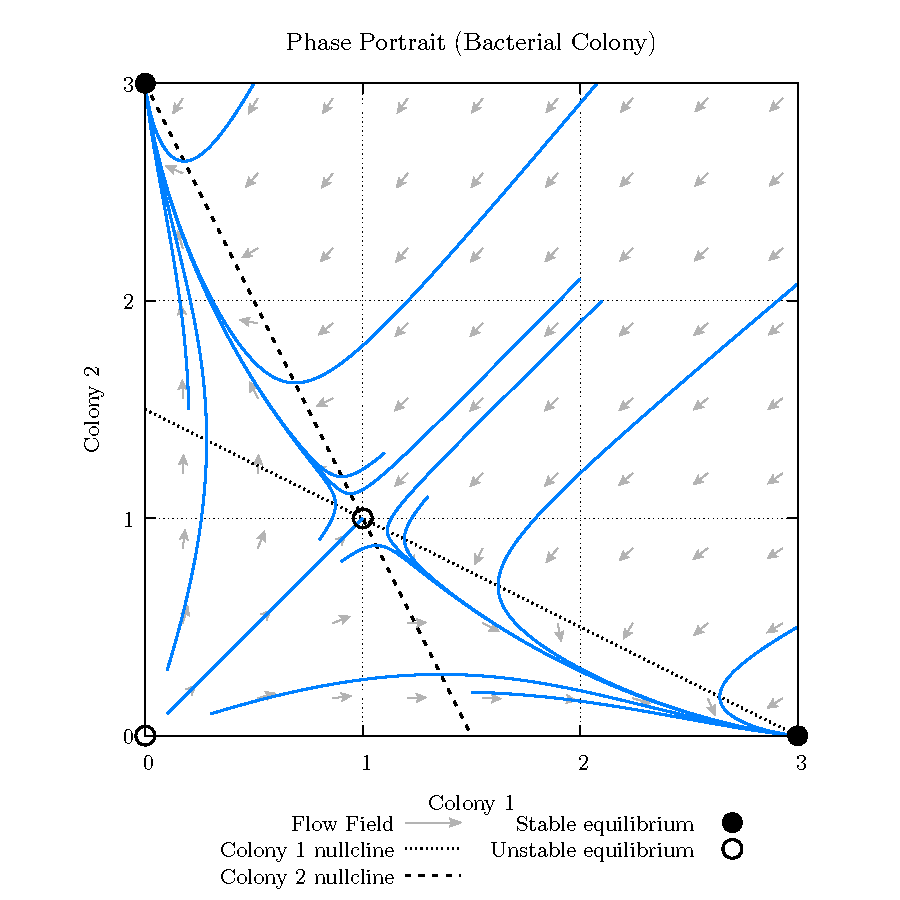
\includegraphics[width=0.8\textwidth]{plots/prob04_bacterial_colony_quiver.pdf}
                \label{fig:prob04_bacterial_model}
            \end{figure}
        \end{itemize}

        \subsection{Problem 5: The Pure Quartic Oscillator}
        \begin{itemize}
            \item {\bf Description:} This models a purely non-linear, conservative mechanical system. Unlike a simple harmonic oscillator, which features a linear restoring force derived from a quadratic potential, the pure quartic oscillator represents a particle trapped in a potential well defined strictly by $V(x) \propto x^4$. Because the linear terms are zero, standard linear stability analysis (Jacobian evaluation) fails at the origin. The phase portrait reveals continuous, closed "squircle" trajectories, demonstrating that the period of oscillation is heavily dependent on the amplitude.
            \item {\bf The Equations:} Using the position $x$ and momentum $y$ (where $y = \dot{x}$), the equations of motion are purely non-linear:
            \begin{eqnarray*}
                \dot{x} & = & y \\
                \dot{y} & = & -x^3
            \end{eqnarray*}
            \item {\bf Code:} \lstinputlisting[style= codestyle]{src/problems/prob05_pure_quartic.f90}
            \item {\bf GNUplot Command:} \lstinputlisting[style= codestyle]{gnuplot/plot_prob05_pure_quartic.plt}
            \item {\bf Plot: }
            \begin{figure}[H]
                \centering
                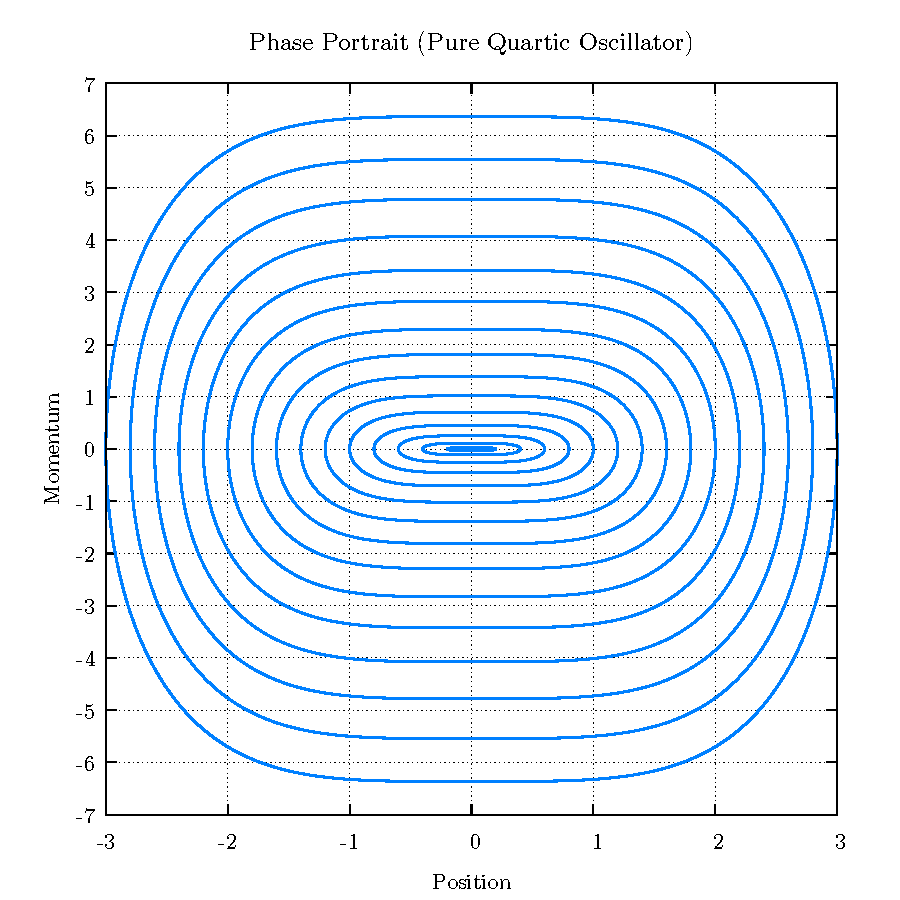
\includegraphics[width=0.8\textwidth]{plots/prob05_pure_quartic.pdf}
                \label{fig:prob05_pure_quartic}
                \end{figure}
        \end{itemize}

        \subsection{Problem 6: The Saddle-Centre Topology}
        \begin{itemize}
            \item {\bf Description:} This dynamical system features a mixture of linear and non-linear terms, creating a complex phase space topology that includes both bounded orbits and unbounded escape trajectories. The linear terms dominate near the equilibria, allowing for standard stability analysis, while the non-linear $-y^2$ term dictates the far-field behavior, causing trajectories outside the stable basin to accelerate toward infinity.
            \item {\bf The Equations:} Using the position $x$ and momentum $y$ (where $y = \dot{x}$), the equations of motion are purely non-linear:
            \begin{eqnarray*}
                \dot{x} & = & x + y - y^2 \\
                \dot{y} & = & x - y
            \end{eqnarray*}
            \item {\bf Code:} \lstinputlisting[style= codestyle]{src/problems/prob06_saddle_centre.f90}
            \item {\bf GNUplot Command:} \lstinputlisting[style= codestyle]{gnuplot/plot_prob06_saddle_centre.plt}
            \item {\bf Plot: }
            \begin{figure}[H]
                \centering
                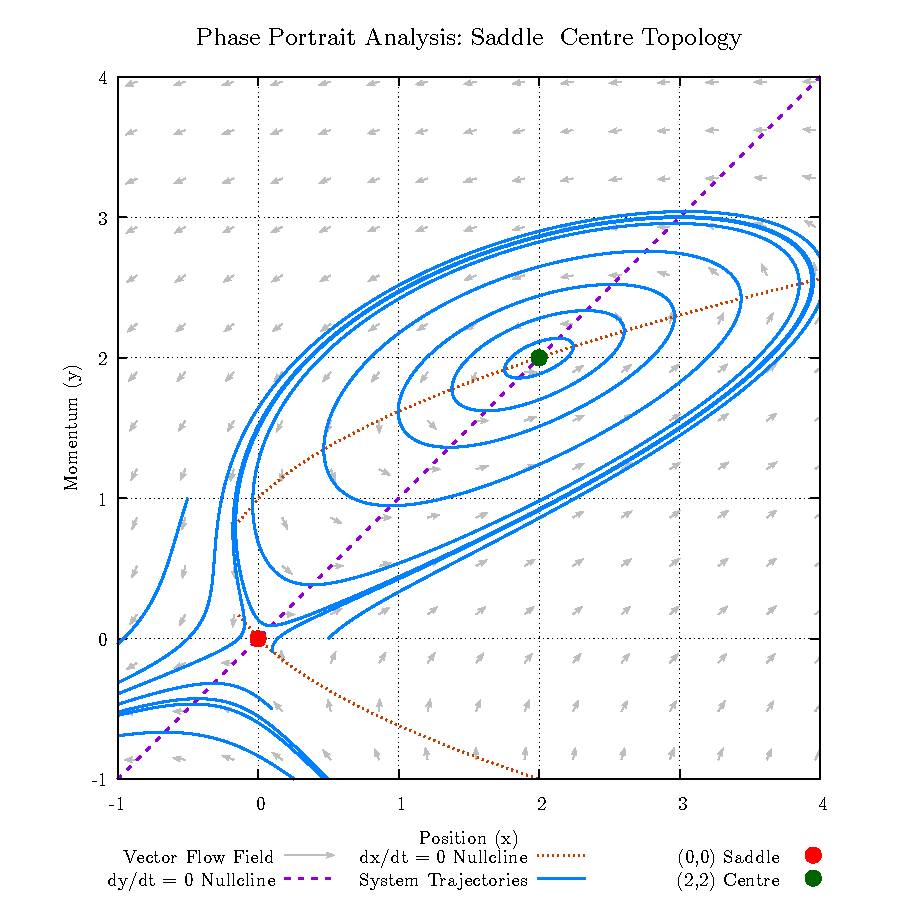
\includegraphics[width=0.8\textwidth]{plots/prob06_dashboard.pdf}
                \label{fig:prob06_saddle_centre}
                \end{figure}
        \end{itemize}

    \section{Remarks}
    The computational exploration of these six dynamical systems highlights the indispensable role of phase portraits in understanding non-linear differential equations. While analytical methods, such as evaluating the Jacobian matrix, successfully predict local behavior near fixed points for systems with linear terms, numerical integration remains a fundamental necessity for uncovering the global dynamics, especially in purely non-linear systems or chaotic regimes.

    Several critical physical and computational observations emerged during this study:
    \begin{itemize}
        \item {\bf Phase Space Topology Dictates Outcomes:} Whether mapping the periodic bounds of the simple pendulum, the chaotic "butterfly" attractor of the Lorenz system, or the rigid $y = x$ separatrix of the symmetric bacterial colony, the phase portrait visually decodes the deterministic fate of the system based on its initial parameters.
        \item {\bf The Limits of Linearization:} The pure Quartic Oscillator proved that in systems completely lacking linear terms, standard Jacobian stability analysis fails entirely. Numerical methods successfully stepped in to reveal that these pure non-linear systems still produce closed, periodic orbits, though their periods are highly dependent on the initial amplitude.
        \item {\bf Sensitivity and Chaos:} The Lorenz system provided a stark contrast to the stable nodes of the Lotka-Volterra models, vividly illustrating how deterministic, non-random equations can produce wildly unpredictable, non-repeating trajectories that are exquisitely sensitive to their starting coordinates.
        \item {\bf Computational Challenges and Solver Limitations:} Using a uniform RK5 solver for the entire assignment exposed a crucial nuance in numerical methods. While RK5 provides exceptional accuracy for general integration, it is not a strictly symplectic integrator. When applied to conservative systems like the pure quartic oscillator and the topological centre, it can introduce artificial numerical dissipation over long integration times. This required careful tuning of the temporal resolution to force the orbits to remain closed. Furthermore, the Saddle-Centre system ($\dot{x} = x + y - y^2$) highlighted the absolute necessity of implementing boundary conditions ("kill switches") in the Fortran code to prevent numerical overflow when simulating trajectories that naturally accelerate to infinity.
    \end{itemize}
    Ultimately, this assignment successfully demonstrates the core pipeline of computational physics: translating complex physical phenomena into coupled differential equations, making active decisions regarding robust numerical algorithms to tame them, and generating information-dense visualizations to interpret the underlying mathematics.
\end{document}